% ============================================================
%  Formation Introductive à Rust
%  Beamer presentation pour Rézoléo faite par Arthur
%  Compilez avec: lualatex --shell-escape formation_rust.tex
%  Dépendances : minted (pip install Pygments), beamer
% ============================================================

\documentclass[aspectratio=169, 10pt]{beamer}

% ---------- THEME & COULEURS --------------------------------
\usetheme{Madrid}
\usecolortheme{default}

% Palette Rust : orange rouille + fond sombre + blanc
\definecolor{RustOrange}{HTML}{CE422B}
\definecolor{RustDark}{HTML}{1C1C1C}
\definecolor{RustLight}{HTML}{F5F0EB}
\definecolor{RustGray}{HTML}{3D3D3D}
\definecolor{RustAccent}{HTML}{F74C00}
\definecolor{SafeGreen}{HTML}{2ECC71}
\definecolor{DangerRed}{HTML}{E74C3C}
\definecolor{NoteBlue}{HTML}{3498DB}
\definecolor{CodeBg}{HTML}{282828}

% Override couleurs Beamer
\setbeamercolor{palette primary}{bg=RustOrange, fg=white}
\setbeamercolor{palette secondary}{bg=RustDark, fg=white}
\setbeamercolor{palette tertiary}{bg=RustGray, fg=white}
\setbeamercolor{palette quaternary}{bg=RustOrange, fg=white}
\setbeamercolor{structure}{fg=RustOrange}
\setbeamercolor{section in toc}{fg=RustDark}
\setbeamercolor{frametitle}{bg=RustDark, fg=white}
\setbeamercolor{title}{fg=white}
\setbeamercolor{subtitle}{fg=RustLight}
\setbeamercolor{author}{fg=RustLight}
\setbeamercolor{date}{fg=RustLight}
\setbeamercolor{titlelike}{parent=palette primary}
\setbeamercolor{block title}{bg=RustOrange, fg=white}
\setbeamercolor{block body}{bg=RustLight, fg=RustDark}
\setbeamercolor{block title alerted}{bg=DangerRed, fg=white}
\setbeamercolor{block body alerted}{bg=red!5, fg=RustDark}
\setbeamercolor{block title example}{bg=SafeGreen!80!black, fg=white}
\setbeamercolor{block body example}{bg=green!5, fg=RustDark}
\setbeamercolor{background canvas}{bg=white}

% ---------- FONTS -------------------------------------------
\usepackage[T1]{fontenc}
\usepackage[utf8]{inputenc}
\usepackage[french]{babel}
\usepackage{lmodern}
\usepackage{microtype}

% ---------- PACKAGES ----------------------------------------
\usepackage{minted}           % code syntax highlighting (nécessite Pygments + --shell-escape)
\usepackage{xcolor}
\usepackage{booktabs}
\usepackage{tabularx}
\usepackage{tikz}
\usetikzlibrary{shapes.geometric, arrows.meta, positioning, fit, backgrounds, decorations.pathreplacing}
\usepackage{fontawesome5}
\usepackage{tcolorbox}
\tcbuselibrary{listings, minted, skins, breakable}
\usepackage{graphicx}
\usepackage{emoji}            % nécessite LuaLaTeX
\usepackage{hyperref}
\hypersetup{colorlinks=true, linkcolor=RustOrange, urlcolor=RustOrange}

% ---------- MINTED CONFIG -----------------------------------
% Style "monokai" sur fond sombre — très lisible en projection
\setminted{
  style=monokai,
  bgcolor=CodeBg,
  fontsize=\footnotesize,
  breaklines=true,
  autogobble=true,
  framesep=2mm,
}

% Shortcut pour inline code Rust
\newmintinline{rust}{style=monokai, bgcolor=CodeBg}

% ---------- TCOLORBOX STYLES --------------------------------
% Box "Règle" orange
\tcbset{
  rulebox/.style={
    enhanced, colback=RustOrange!10, colframe=RustOrange,
    fonttitle=\bfseries, coltitle=white, attach boxed title to top left,
    boxed title style={colback=RustOrange, rounded corners},
    rounded corners, top=0mm, bottom=0mm, left=0mm, right=0mm
  },
  dangerbox/.style={
    enhanced, colback=DangerRed!8, colframe=DangerRed,
    fonttitle=\bfseries, coltitle=white, attach boxed title to top left,
    boxed title style={colback=DangerRed, rounded corners},
    rounded corners, top=0mm, bottom=0mm, left=0mm, right=0mm
  },
  safebox/.style={
    enhanced, colback=SafeGreen!8, colframe=SafeGreen!70!black,
    fonttitle=\bfseries, coltitle=white, attach boxed title to top left,
    boxed title style={colback=SafeGreen!70!black, rounded corners},
    rounded corners, top=0mm, bottom=0mm, left=0mm, right=0mm
  },
  notebox/.style={
    enhanced, colback=NoteBlue!8, colframe=NoteBlue,
    fonttitle=\bfseries, coltitle=white, attach boxed title to top left,
    boxed title style={colback=NoteBlue, rounded corners},
    rounded corners, top=0mm, bottom=0mm, left=0mm, right=0mm
  }
}

% ---------- BEAMER MISC -------------------------------------
\setbeamertemplate{navigation symbols}{}   % pas de boutons nav
\setbeamertemplate{itemize items}[circle]
\setbeamercolor{itemize item}{fg=RustOrange}
\setbeamercolor{itemize subitem}{fg=RustGray}
\setbeamerfont{frametitle}{series=\bfseries}

% Pied de page
\setbeamertemplate{footline}{%
  \leavevmode%
  \hbox{%
    \begin{beamercolorbox}[wd=.5\paperwidth, ht=2.5ex, dp=1.5ex, left, leftskip=1em]{palette secondary}%
      \usebeamerfont{author in head/foot}\insertshorttitle
    \end{beamercolorbox}%
    \begin{beamercolorbox}[wd=.5\paperwidth, ht=2.5ex, dp=1.5ex, right, rightskip=1em]{palette primary}%
      \usebeamerfont{author in head/foot}\insertframenumber{} / \inserttotalframenumber
    \end{beamercolorbox}%
  }%
}

% ---------- COMMANDES UTILES --------------------------------
\newcommand{\CC}{C\nolinebreak\hspace{-.05em}\raisebox{.3ex}{\scriptsize\bfseries +}\nolinebreak\hspace{-.10em}\raisebox{.3ex}{\scriptsize\bfseries +}}
\newcommand{\rust}[1]{\mintinline{rust}{#1}}
\newcommand{\ccode}[1]{\mintinline{c}{#1}}
\newcommand{\bash}[1]{\mintinline{bash}{#1}}
\newcommand{\keyword}[1]{{\color{RustOrange}\textbf{#1}}}
\newcommand{\safe}{{\color{SafeGreen}\faCheckCircle\ \textbf{SAFE}}}
\newcommand{\unsafe}{{\color{DangerRed}\faTimesCircle\ \textbf{UNSAFE}}}
\newcommand{\compilerr}{{\color{DangerRed}\faTimesCircle\ \textbf{ERREUR COMPILATION}}}
\newcommand{\compilerok}{{\color{SafeGreen}\faCheckCircle\ \textbf{COMPILE OK}}}

% ============================================================
%  MÉTADONNÉES
% ============================================================
\title[Introduction à Rust]{\huge\textbf{Introduction à Rust}}
\subtitle{Pourquoi un nouveau langage systèmes en 2026~?}
\author{Arthur Chollet}
\institute{Rézoléo}
\date{\today}

% ============================================================
%  DÉBUT DU DOCUMENT
% ============================================================
\begin{document}

% -------- TITLE SLIDE ---------------------------------------
{
\setbeamercolor{background canvas}{bg=RustDark}
\begin{frame}[plain]
  \vspace{1.5em}
  \begin{center}
    {\color{RustOrange}\fontsize{40}{48}\selectfont\textbf{\faRust}} \\[0.3em]
    {\color{white}\fontsize{28}{34}\selectfont\textbf{Introduction à Rust}}\\[0.3em]
    {\color{RustLight}\large Pourquoi un nouveau langage systèmes en 2026~?}\\[1.5em]
    {\color{RustLight}\normalsize Arthur \textbar\ Rézoléo \textbar\ \today}
  \end{center}

  \begin{columns}[t]
    \column{0.5\textwidth}
    \begin{center}
      
\includegraphics[height=2cm]{Img/ferris.png}
    \end{center}
    \column{0.5\textwidth}
    \begin{center}
      
\includegraphics[height=2cm]{Img/ferris.png}
    \end{center}
  \end{columns}
\end{frame}
}

% -------- PLAN ----------------------------------------------
\begin{frame}{Au programme}
  \begin{columns}[t]
    \column{0.55\textwidth}
    \tableofcontents[hideallsubsections]
    \column{0.42\textwidth}
    \begin{tcolorbox}[notebox, title={\faInfoCircle\ Objectif}]
      \small
      Comprendre \textbf{pourquoi} Rust existe et ce qui le rend unique.\\[0.5em]
      Prérequis~: vous connaissez \textbf{le C}.
    \end{tcolorbox}
    \begin{center}
      
\includegraphics[height=4cm]{Img/universe_rust.png}
    \end{center}
  \end{columns}
\end{frame}

% ============================================================
\section{Motivation}
% ============================================================

\begin{frame}{La stat qui fait mal au puriste du C}
  \begin{columns}[c]
    \column{0.52\textwidth}
    \begin{tcolorbox}[dangerbox, title={\faExclamationTriangle\ Chiffres réels}]
      \large
      \begin{itemize}
        \item \textbf{\color{DangerRed}$\sim$70\%} des CVE dans Chrome\\
              $\to$ bugs \textbf{mémoire}
        \item \textbf{\color{DangerRed}$\sim$70\%} des CVE Windows\\
              $\to$ idem (Microsoft, 2019)
        \item \textbf{\color{DangerRed}$\sim$65\%} des CVE Android\\
              $\to$ idem (Google, 2019)
      \end{itemize}
    \end{tcolorbox}

    \column{0.45\textwidth}
    \vspace{2em}
    \begin{tcolorbox}[colback=RustLight, colframe=RustGray]
      \centering
      \begin{tikzpicture}[scale=0.9]
      \draw (0,0) circle (1.4cm);  % Optional outline
      \fill[DangerRed!90] (0,0) -- (-162:1.4cm) arc(-162:90:1.4cm) -- cycle;
      \fill[RustGray!60]  (0,0) -- (-162:1.4cm) arc(-162:-270:1.4cm) -- cycle;
        \node[font=\tiny\bfseries, color=white] at (-0.3, 0.1) {30\%};
        \node[font=\tiny, color=RustDark] at (0.3, -0.5) {70\%};
        \node[font=\tiny\bfseries, color=DangerRed] at (0, -1.9) {Bugs mémoire};
        \node[font=\tiny, color=RustGray] at (0, -2.3) {Autres CVE};
      \end{tikzpicture}
    \end{tcolorbox}
  \end{columns}
  \vspace{0.5em}
  \begin{center}
    \large\textit{``On connaît le C depuis 50 ans, on a Valgrind, ASan, code reviews~--- \textbf{pourquoi ça continue~?}''}
  \end{center}
\end{frame}

\begin{frame}{Qu'est-ce que Rust~?}
  \begin{columns}[t]
    \column{0.5\textwidth}
    \begin{block}{Globalement}
      Langage \textbf{systèmes compilé}, \textbf{statiquement typé}, \textbf{sans GC}, qui rend les bugs mémoire \textbf{impossibles à compiler}.
    \end{block}
    \vspace{0.5em}
    \begin{itemize}
      \item Né chez \textbf{Mozilla Research} $\sim$2010
      \item Objectif~: réécrire Firefox sans bugs \CC
      \item Grande communauté (cargo, crates.io ...)
      \item Stable depuis \textbf{2015}, ajd: edition 2024 (3ans)
      \item Aujourd'hui~: Linux kernel, Android, Windows, AWS, Cloudflare, Discord\ldots
      \item \faHeart\ \textbf{10 ans} consécutifs ``Most Loved Language'' (SO Survey)
    \end{itemize}

    \column{0.47\textwidth}
    \begin{tcolorbox}[rulebox]
      \footnotesize
      \begin{tabular}{@{}lp{4.7cm}@{}}
        \toprule
        \textbf{Langage} & \textbf{Trade-off} \\
        \midrule
        C / \CC  & Rapide, mais \unsafe \\[3pt]
        Java / Go & \safe, mais GC (pause, overhead) \\[3pt]
        \textbf{Rust} & \safe\ \textbf{+} rapide, \textbf{sans GC} \\
        \bottomrule
      \end{tabular}
    \end{tcolorbox}
    % \begin{tcolorbox}[notebox, title={\faLightbulb\ Bref}]
    %   
    % \end{tcolorbox}
    \begin{center}
      
\includegraphics[height=3.9cm]{Img/racelang.jpg}
    \end{center}
  \end{columns}
\end{frame}

% ============================================================
\section{Le problème du C}
% ============================================================

\begin{frame}[fragile]{Ces bugs mémoire en C sont ridicules, mais même Torvalds en fait}
  \begin{columns}[t]
    \column{0.48\textwidth}
    \begin{tcolorbox}[dangerbox, title={\faSkull\ Use-after-free}]
      \begin{minted}[fontsize=\scriptsize]{c}
int *p = malloc(sizeof(int));
free(p);
*p = 42; // UB — le compilo dit rien
      \end{minted}
    \end{tcolorbox}
    \vspace{0.3em}
    \begin{tcolorbox}[dangerbox, title={\faSkull\ Double free}]
      \begin{minted}[fontsize=\scriptsize]{c}
free(p);
free(p); // crash ou corruption silencieuse
      \end{minted}
    \end{tcolorbox}
    \column{0.48\textwidth}
    \begin{tcolorbox}[dangerbox, title={\faSkull\ Buffer overflow}]
      \begin{minted}[fontsize=\scriptsize]{c}
char buf[8];
strcpy(buf, "hello world"); // écrase la stack
      \end{minted}
    \end{tcolorbox}
    \vspace{0.3em}
    \begin{tcolorbox}[dangerbox, title={\faSkull\ Data race (multi-thread)}]
      \begin{minted}[fontsize=\scriptsize]{c}
// Thread 1 et Thread 2 modifient
// la même variable sans mutex.
// Le compilateur C : ¯\_(?)_/¯
      \end{minted}
    \end{tcolorbox}
  \end{columns}
\end{frame}

\begin{frame}[fragile]{Ces bugs mémoire en C sont ridicules, mais même Torvalds en fait}
  \begin{columns}[t]
    \column{0.6\textwidth}
    \begin{tcolorbox}[dangerbox, title={\faSkull\ Dangling pointer}]
      \begin{minted}[fontsize=\scriptsize]{c}
int* get_val() {
    int x = 5;
    return &x; // x est sur la stack, elle sera détruite
}
      \end{minted}
    \end{tcolorbox}
    \vspace{0.3em}
    \begin{tcolorbox}[safebox, title={\faRust\ Rust}]
      \small Ces \textbf{5 classes de bugs} sont \textbf{impossibles à compiler} en Rust. Car Rust \textbf{déplace} la vérification de la sécurité mémoire du \textit{runtime} vers le \textbf{compile time}.
    \end{tcolorbox}
    \column{0.4\textwidth}
    \vspace{2em}
    \begin{center}
      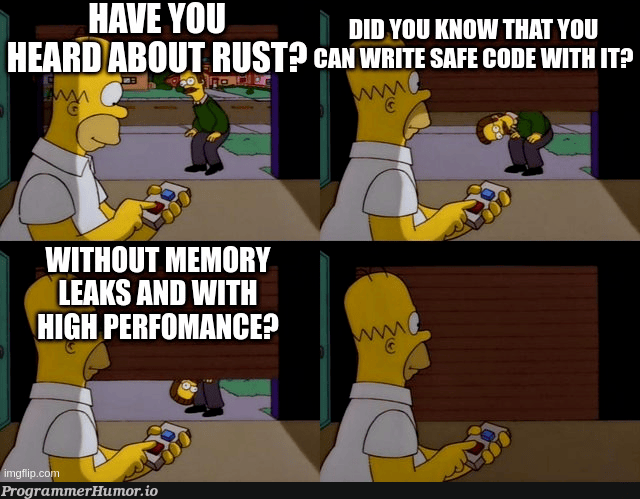
\includegraphics[height=4cm]{Img/homerrust.png}
    \end{center}
  \end{columns}
  \vspace{1em}
  \begin{center}
     {\footnotesize\color{RustGray} (Valgrind, ASan, Tsan détectent \textit{après}, pas toujours en prod. Rust refusera de \textit{compiler}.)}
  \end{center}
\end{frame}

% ============================================================
\section{Ownership \& RAII}
% ============================================================

\begin{frame}{Stack vs Heap --- rappel}
  \begin{columns}[c]
    \column{0.48\textwidth}
    \begin{tikzpicture}[scale=1, every node/.style={font=\small}]
      % Stack
      \foreach \i/\c in {0/RustGray!30, 1/RustGray!50, 2/RustOrange!60, 3/RustOrange!80} {
        \draw[fill=\c, draw=RustDark] (0, \i*0.6) rectangle (1.8, \i*0.6+0.5);
      }
      \node[above, font=\footnotesize\bfseries, color=RustDark] at (0.9, 2.5) {Stack};
      \draw[->, thick, RustOrange] (0.9, 2.4) -- (0.9, 2.0);
      \node[right, font=\tiny, color=RustGray] at (1.9, 1.0) {libération};
      \node[right, font=\tiny, color=RustGray] at (1.9, 0.6) {automatique};

      % Heap
      \foreach \pos in {(3,0.2), (3.8,1.1), (3.2,2.0), (4.5,0.7)} {
        \draw[fill=NoteBlue!40, draw=RustDark, rounded corners=2pt] \pos rectangle ++(0.7,0.45);
      }
      \node[above, font=\footnotesize\bfseries, color=RustDark] at (3.85, 2.6) {Heap};
      \node[below, font=\tiny, color=DangerRed, align=center] at (3.85, -0.1) {tu gères\\(malloc/free)};
    \end{tikzpicture}

    \column{0.48\textwidth}
    \begin{itemize}
      \item \textbf{Stack} : taille connue à la compilation,\\libération automatique en sortant du scope.
      \vspace{0.4em}
      \item \textbf{Heap} : \ccode{malloc}/\ccode{free} en C,\\taille dynamique, \textbf{TU es responsables}.
      \vspace{0.4em}
      \item Le problème : ce \textit{``tu es responsables''}\\que Rust automatise \textbf{sans GC}.
    \end{itemize}
  \end{columns}
\end{frame}

\begin{frame}[fragile]{RAII --- Resource Acquisition Is Initialization}
  \begin{columns}[t]
    \column{0.48\textwidth}
    \begin{block}{\CC\ (smart pointers)}
      \begin{minted}[fontsize=\scriptsize]{cpp}
{
    auto p = std::make_unique<int>(42);
    // p alloué ici
} // p détruit ici — mémoire libérée
      \end{minted}
    \end{block}
    Concept né en \CC\ (Bjarne Stroustrup).\\
    Opt-in : il faut choisir \mintinline{cpp}{unique_ptr}.

    \column{0.48\textwidth}
    \begin{tcolorbox}[safebox, title={\faRust\ Rust --- comportement \textbf{par défaut}}]
      \begin{minted}[fontsize=\scriptsize]{rust}
{
    let s = String::from("hello");
    // alloué sur le heap
} // `drop(s)` inséré par le compilateur
  // → mémoire libérée automatiquement
      \end{minted}
    \end{tcolorbox}
    \begin{tcolorbox}[notebox]
      \small \textbf{Zéro overhead runtime.}\\
      Le compilateur insère \rust{drop()} à la compilation.\\
      Pas de GC. Pas de \ccode{free}. Déterministe.
    \end{tcolorbox}
  \end{columns}
\end{frame}

\begin{frame}{Les 3 règles d'Ownership}
  \begin{center}
    \begin{tcolorbox}[rulebox, title={\faBook\ Les règles fondamentales de Rust}, width=0.92\textwidth]
      \large
      \begin{enumerate}
        \setlength\itemsep{0.6em}
        \item Chaque valeur a \textbf{un seul owner} (propriétaire).
        \item Il ne peut y avoir \textbf{qu'un seul owner à la fois}.
        \item Quand l'owner sort du scope, la valeur est \textbf{détruite}.
      \end{enumerate}
    \end{tcolorbox}
  \end{center}
  \vspace{0.5em}
  \begin{columns}[c]
    \column{0.5\textwidth}
    \begin{tcolorbox}[notebox]
      \small En C, deux pointeurs peuvent pointer vers la même zone mémoire~--- source de \textbf{tous} les bugs précédents.\\[0.4em]
      En Rust, \textbf{par construction}, une seule variable est propriétaire à tout moment.
    \end{tcolorbox}
    \column{0.47\textwidth}
    \begin{tikzpicture}[scale=1, every node/.style={font=\small}]
      % Avant move
      \node[draw=RustOrange, fill=RustOrange!15, rounded corners, minimum width=1.2cm, minimum height=0.6cm] (s1) at (0,1.5) {\texttt{s1}};
      \node[draw=NoteBlue, fill=NoteBlue!15, rounded corners, minimum width=1.6cm, minimum height=0.6cm] (heap) at (2.8,1.5) {\texttt{"hello"}};
      \draw[->, thick, RustOrange] (s1) -- (heap) node[midway, above, font=\tiny] {owner};

      % Après move
      \node[draw=DangerRed, fill=DangerRed!10, rounded corners, minimum width=1.2cm, minimum height=0.6cm, opacity=0.5] (s1b) at (0,0) {\texttt{s1}};
      \draw[DangerRed, very thick] (-0.6,-0.3) -- (0.6,0.3);
      \node[draw=SafeGreen!70!black, fill=SafeGreen!15, rounded corners, minimum width=1.2cm, minimum height=0.6cm] (s2) at (1.5,0) {\texttt{s2}};
      \draw[->, thick, SafeGreen!70!black] (s2) -- (heap);
      \node[below, font=\tiny, color=DangerRed] at (0,-0.5) {invalide};
      \node[below, font=\tiny, color=SafeGreen!70!black] at (1.5,-0.5) {owner};
      \node[above, font=\tiny\bfseries] at (1.5, 2.1) {Move~: \texttt{let s2 = s1}};
    \end{tikzpicture}
  \end{columns}
\end{frame}

\begin{frame}[fragile]{Move semantics --- C vs Rust}
  \begin{columns}[t]
    \column{0.48\textwidth}
    \begin{tcolorbox}[dangerbox, title={C --- deux pointeurs}]
      \begin{minted}[fontsize=\scriptsize]{c}
char *s1 = malloc(6);
strcpy(s1, "hello");
char *s2 = s1; // copie du pointeur

free(s1);
// s2 pointe vers mémoire libérée
// → dangling pointer silencieux !
printf("%s\n", s2); // UB
      \end{minted}
    \unsafe
    \end{tcolorbox}

    \column{0.48\textwidth}
    \begin{tcolorbox}[safebox, title={\faRust\ Rust --- move interdit de réutiliser}]
      \begin{minted}[fontsize=\scriptsize]{rust}
let s1 = String::from("hello");
let s2 = s1; // s1 est "moved" dans s2

// s1 est maintenant invalide
println!("{}", s1);
// error[E0382]: borrow of moved value
      \end{minted}
    \compilerr
    \end{tcolorbox}
  \end{columns}
  \begin{tcolorbox}[notebox, title={\faLightbulb\ Copy vs Move}]
    \small
    \textbf{Types primitifs} (\rust{i32}, \rust{bool}, \rust{f64}\ldots) = \textbf{Copy} comme en C.\\
    \textbf{Types heap} (\rust{String}, \rust{Vec}\ldots) = \textbf{Move}~: transfert de propriété, pas copie profonde.\\
    Copie explicite~: \rust{s1.clone()} (coûteux, et c'est \textbf{intentionnel}... c'est une mauvaise pratique en rust).
  \end{tcolorbox}
\end{frame}

\begin{frame}[fragile]{Move error exemple}
   \begin{columns}[t]
    \column{0.7\textwidth}
    \begin{tcolorbox}[dangerbox, title={\faTerminal\ Message du compilateur}]
      \color{white}
      \begin{minted}[fontsize=\tiny, bgcolor=RustDark]{text}
$ cargo run
   Compiling ownership v0.1.0 (file:///projects/ownership)
error[E0382]: borrow of moved value: `s1`
 --> src/main.rs:5:16
  |
2 |     let s1 = String::from("hello");
  |         -- move occurs because `s1` has type `String`, which does not implement the `Copy` trait
3 |     let s2 = s1;
  |              -- value moved here
4 |
5 |     println!("{s1}, world!");
  |                ^^ value borrowed here after move
  |
  = note: this error originates in the macro `$crate::format_args_nl` which comes from the expansion of the macro `println` (in Nightly builds, run with -Z macro-backtrace for more info)
help: consider cloning the value if the performance cost is acceptable
  |
3 |     let s2 = s1.clone();
  |                ++++++++

For more information about this error, try `rustc --explain E0382`.
error: could not compile `ownership` (bin "ownership") due to 1 previous error
      \end{minted}
    \end{tcolorbox}
    \column{0.3\textwidth}
    \vspace{1.9em}
    \begin{tcolorbox}[dangerbox]
      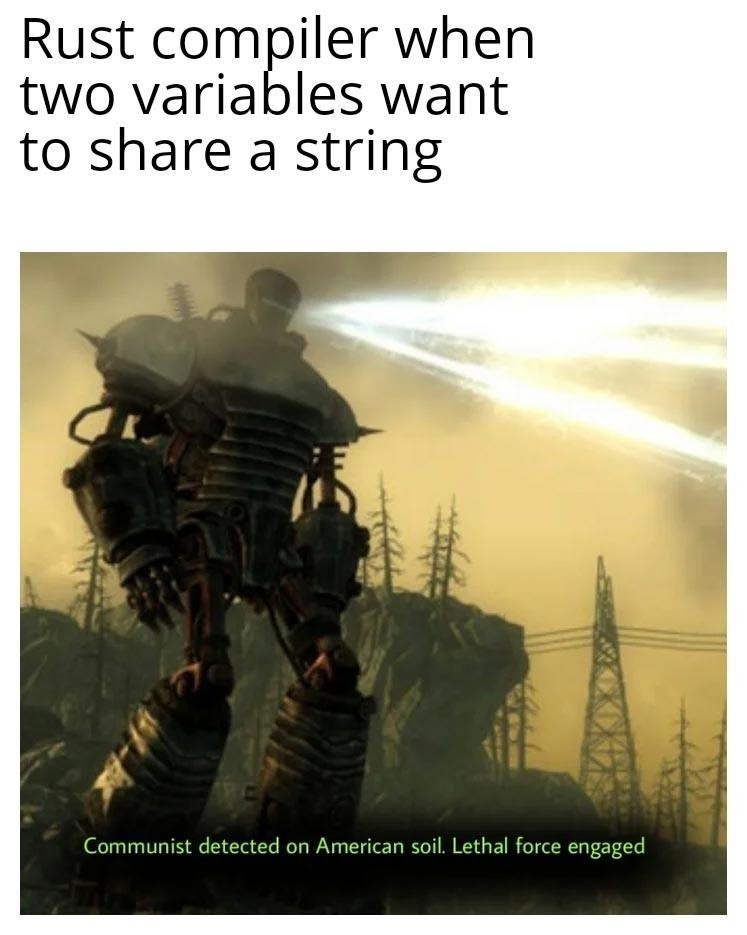
\includegraphics[height=5cm]{Img/communist_rust.jpeg}
    \end{tcolorbox}
  \end{columns}
\end{frame}

\begin{frame}{Ownership vs GC ??}
  \begin{columns}[c]
    \column{0.48\textwidth}
    \begin{tcolorbox}[dangerbox, title={\faTrash\ GC (Java, Go, Python\ldots)}]
      \begin{itemize}\small
        \item Traque les références \textbf{au runtime}
        \item Pauses GC imprévisibles (``stop-the-world'')
        \item Overhead mémoire ($\times$2--5)
        \item Non-déterministe~: vous ne savez pas \textit{quand} les ressources sont libérées
      \end{itemize}
    \end{tcolorbox}

    \column{0.48\textwidth}
    \begin{tcolorbox}[safebox, title={\faRust\ Rust --- Ownership at compile time}]
      \begin{itemize}\small
        \item Traque la propriété \textbf{à la compilation}
        \item Libération \textbf{déterministe}~: à la fermeture du scope
        \item Zéro overhead runtime
        \item Performances comparables voir supérieur à C/\CC\, \textit{si bien écrit}
      \end{itemize}
    \end{tcolorbox}
  \end{columns}
  \vspace{0.7em}
  \begin{center}
    \begin{tcolorbox}[rulebox, title={\faRust\ La promesse de Rust}, width=0.85\textwidth]
      \centering\large
      \textbf{Même vitesse que C} \faPlus\ \textbf{zéro bug mémoire}\\[0.3em]
      \small Le compilateur fait le travail à ta place.
    \end{tcolorbox}
  \end{center}
\end{frame}

% ============================================================
\section{Borrowing \& Borrow Checker}
% ============================================================

\begin{frame}[fragile]{En pratique: le Borrowing \& Borrow Checker}
  \begin{columns}[t]
    \column{0.52\textwidth}
    \begin{tcolorbox}[dangerbox, title={\faQuestion\ Problème: Move est trop restrictif}]
      \begin{minted}[fontsize=\scriptsize]{rust}
fn print_len(s: String) { // prend ownership
    println!("{}", s.len());
} // s est droppé ici !

let s = String::from("hello");
print_len(s); // ownership moved
println!("{}", s); // ERREUR : s invalide
      \end{minted}
      \compilerr
    \end{tcolorbox}

    \column{0.44\textwidth}
    \vspace{1em}
    \begin{tcolorbox}[notebox, title={\faBalanceScale\ Solution~: emprunter}]
      \small
      Passer une \textbf{référence} à la fonction~---\\
      elle \textit{emprunte} sans prendre la propriété.\\[0.5em]
      Comme un \ccode{const *} en C\ldots\\
      mais avec des \textbf{garanties formelles}.
    \end{tcolorbox}
    \begin{center}
      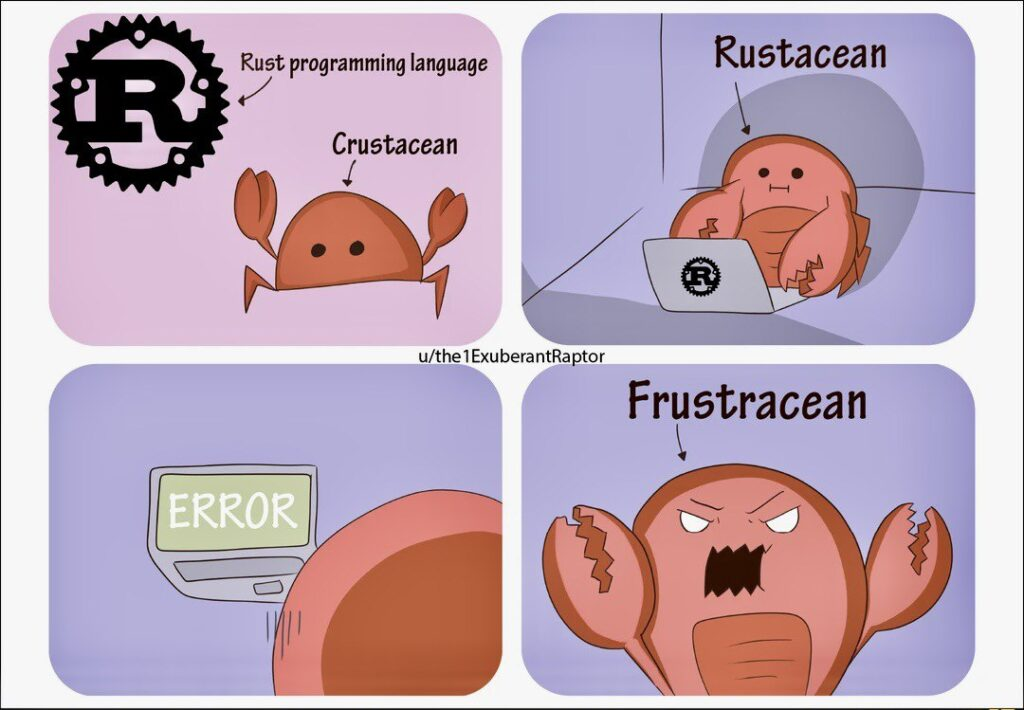
\includegraphics[height=3.5cm]{Img/frustacean.jpg}
    \end{center}
  \end{columns}
\end{frame}

\begin{frame}[fragile]{Borrowing --- \&T et \&mut T}
  \begin{columns}[t]
    \column{0.50\textwidth}
    \begin{tcolorbox}[safebox, title={\faRust\ Référence immuable \texttt{\&T}}]
      \begin{minted}[fontsize=\scriptsize]{rust}
fn print_len(s: &String) { // emprunte
    println!("{}", s.len());
} // rien n'est droppé

let s = String::from("hello");
print_len(&s); // on prête s
println!("{}", s); // OK : s est toujours là
      \end{minted}
    \compilerok
    \end{tcolorbox}

    \column{0.46\textwidth}
    \begin{tcolorbox}[rulebox, title={\faBook\ Règles du Borrow Checker}]
      \small À tout instant, vous pouvez avoir
      \begin{itemize}
        \item \textbf{Soit} autant de \rust{&T} que vous voulez\\{\tiny (lecture seule, pas de modification)}
        \item \textbf{Soit} exactement \textbf{un} \rust{&mut T}\\{\tiny (écriture exclusive)}
      \end{itemize}
      \textbf{jamais les deux en même temps.}
    \end{tcolorbox}
  \end{columns}
  \begin{tcolorbox}[notebox, title={\faLightbulb\ Pourquoi~?}]
    \small \textbf{Plusieurs lecteurs~:} pas de modification~=~pas de corruption.\\
    \textbf{Un seul écrivain~:} personne d'autre ne lit pendant l'écriture~=~pas de data race.\\
    \textbf{Lecteur + écrivain~:} UB en C~--- \textbf{impossible à compiler} en Rust.
  \end{tcolorbox}
\end{frame}

\begin{frame}[fragile]{Borrow Checker en action --- erreur de violation}
  \begin{columns}[t]
    \column{0.52\textwidth}
    \begin{tcolorbox}[dangerbox, title={\faSkull\ Code Rust invalide}]
      \begin{minted}[fontsize=\scriptsize]{rust}
let mut v = vec![1, 2, 3];
let first = &v[0]; // emprunt immuable
v.push(4);         // ERREUR : emprunt mutable
                   // alors que first existe
println!("{}", first);
      \end{minted}
    \end{tcolorbox}
    \begin{tcolorbox}[dangerbox, title={\faTerminal\ Message du compilateur}]
      \color{white}
      \begin{minted}[fontsize=\tiny, bgcolor=RustDark]{text}
error[E0502]: cannot borrow `v` as mutable
   --> src/main.rs:3:1
    |
2   | let first = &v[0];
    |              - immutable borrow here
3   | v.push(4);
    | ^^^^^^^^^ mutable borrow here
4   | println!("{}", first);
    |                ----- used here
      \end{minted}
    \end{tcolorbox}

    \column{0.44\textwidth}
    \begin{tcolorbox}[dangerbox, title={En C~: skill issue}]
      \begin{minted}[fontsize=\scriptsize]{c}
int *arr = malloc(3 * sizeof(int));
int *first = &arr[0];
// realloc peut déplacer le tableau !
arr = realloc(arr, 4 * sizeof(int));
// first est maintenant un dangling
// pointer. Aucune erreur.
printf("%d\n", *first); // UB
      \end{minted}
    \end{tcolorbox}
  \end{columns}
\end{frame}

\begin{frame}[fragile]{Le Borrow Checker: ami pour la vie ?}
  \begin{columns}[t]
    \column{0.5\textwidth}
    \begin{tcolorbox}[notebox]
      \small Le borrow checker \textbf{n'est pas ton ennemi}.\\
      Il a \textbf{toujours raison} et tu es son esclave.
    \end{tcolorbox}
  \end{columns}
  \begin{columns}[t]
    \column{0.5\textwidth}
    \begin{center}
      
\includegraphics[height=5cm]{Img/rustcompiler.png}
    \end{center}
    \column{0.5\textwidth}
    \begin{center}
      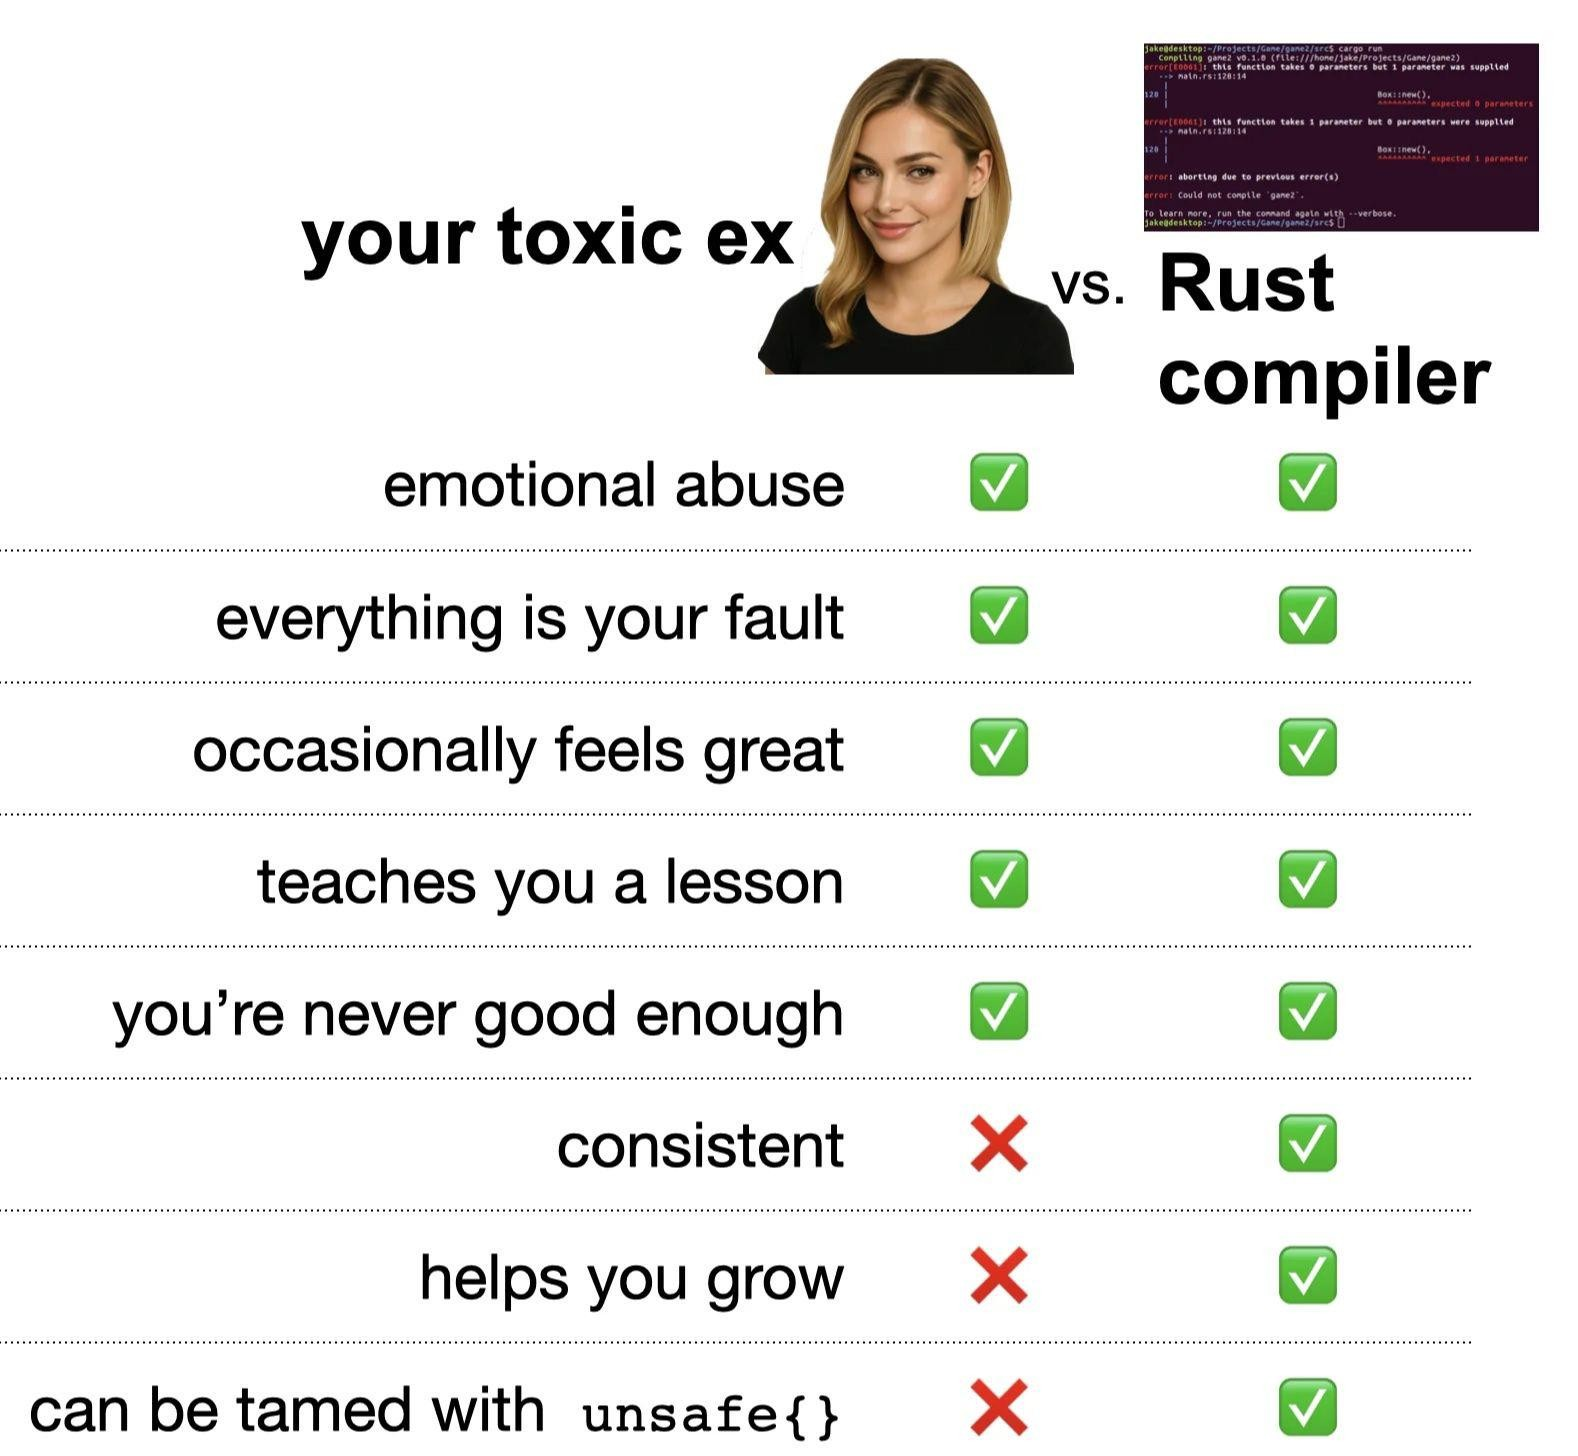
\includegraphics[height=5cm]{Img/toxicex.jpeg}
    \end{center}
  \end{columns}
\end{frame}


\begin{frame}[fragile]{Lifetimes --- les références ne peuvent pas ``survivre'' leurs données}
  \begin{columns}[t]
    \column{0.50\textwidth}
    \begin{tcolorbox}[dangerbox, title={\faSkull\ C~: dangling pointer silencieux}]
      \begin{minted}[fontsize=\scriptsize]{c}
int* get() {
    int x = 5;
    return &x; // x va mourir !
} // UB
      \end{minted}
    \end{tcolorbox}
    \vspace{0.3em}
    \begin{tcolorbox}[safebox, title={\faRust\ Rust~: erreur de compilation}]
      \begin{minted}[fontsize=\scriptsize]{rust}
fn get() -> &i32 {
    let x = 5;
    &x
// error: `x` does not live long enough
}
      \end{minted}
    \end{tcolorbox}

    \column{0.46\textwidth}
    \begin{tcolorbox}[notebox, title={\faBook\ Concept de Lifetime}]
      \small
      Chaque référence a une \textbf{lifetime}~: la durée de vie de la donnée pointée.\\[0.5em]
      Le compilateur vérifie que \textbf{la référence ne survit jamais} à la donnée.\\[0.5em]
      Dans 95\% des cas~: inféré automatiquement.\\[0.5em]
      Les annotations \rust{'a} n'apparaissent qu'en cas d'ambiguïté.
    \end{tcolorbox}
    \vspace{0.3em}
    \begin{tcolorbox}[safebox, title={\faCheckCircle\ Garantie}]
      \small Si ça compile~:\\
      \textbf{aucun dangling pointer n'est possible.}
    \end{tcolorbox}
  \end{columns}
\end{frame}

\begin{frame}[fragile]{Les lifetimes}
  \begin{columns}[t]
    \column{0.6\textwidth}
    \begin{tcolorbox}[safebox, title={\faRust\ Concrétement}]
      \begin{minted}[fontsize=\scriptsize]{rust}
fn main() {
    let r;                // ---------+-- 'a
                          //          |
    {                     //          |
        let x = 5;        // -+-- 'b  |
        r = &x;           //  |       |
    }                     // -+       |
                          //          |
    println!("r: {r}");   //          |
}                         // ---------+
      \end{minted}
    \end{tcolorbox}
    \column{0.4\textwidth}
    \begin{center}
      
\includegraphics[height=5cm]{Img/sanity.jpeg}
    \end{center}
  \end{columns}
\end{frame}

\begin{frame}{Résumé~: ce que le compilateur garantit}
  \begin{center}
    \begin{tabular}{lccc}
      \toprule
      \textbf{Garantie} & \textbf{C} & \textbf{\CC\ moderne} & \textbf{Rust} \\
      \midrule
      Rapide (0 overhead) & {\color{SafeGreen}\faCheck} & {\color{SafeGreen}\faCheck} & {\color{SafeGreen}\faCheck} \\
      No use-after-free & {\color{DangerRed}\faTimes} & {\color{NoteBlue}\small opt-in} & {\color{SafeGreen}\faCheck} \\
      No double-free     & {\color{DangerRed}\faTimes} & {\color{NoteBlue}\small opt-in} & {\color{SafeGreen}\faCheck} \\
      No dangling pointer & {\color{DangerRed}\faTimes} & {\color{NoteBlue}\small opt-in} & {\color{SafeGreen}\faCheck} \\
      No buffer overflow  & {\color{DangerRed}\faTimes} & {\color{DangerRed}\faTimes} & {\color{SafeGreen}\faCheck} \\
      No data race        & {\color{DangerRed}\faTimes} & {\color{DangerRed}\faTimes} & {\color{SafeGreen}\faCheck} \\
      \bottomrule
    \end{tabular}
    \vspace{0.5em}
    \begin{tcolorbox}[rulebox, title={}, width=0.85\textwidth]
      \centering
      En Rust~: pas de GC, pas de runtime, \textbf{toutes les garanties encodées dans le compilateur}.
    \end{tcolorbox}
  \end{center}
\end{frame}

% ============================================================
\section{Syntaxe \& Forces Expressives}
% ============================================================

\begin{frame}[fragile]{Les types de bases}
  \begin{columns}[t]
    \column{0.6\textwidth}
    \begin{tcolorbox}[safebox, title={\faRust\ Types primitifs}]
      \begin{minted}[fontsize=\scriptsize]{rust}
        i8, i16, i32, i64, i128, isize
        u8, u16, u32, u64, u128, usize
        f32, f64
        bool
        char = 'a'
        let (a,b,c): (i32, f64, u8) = (500, 6.4, 1);
        let [a,b,..]: [i32; 5] = [-1, 2, -3, 4, -5];
        str -> let g_pas_didee_de_nom: &str = "hello";
        ()
      \end{minted}
    \end{tcolorbox}
    \column{0.4\textwidth}
    \begin{center}
      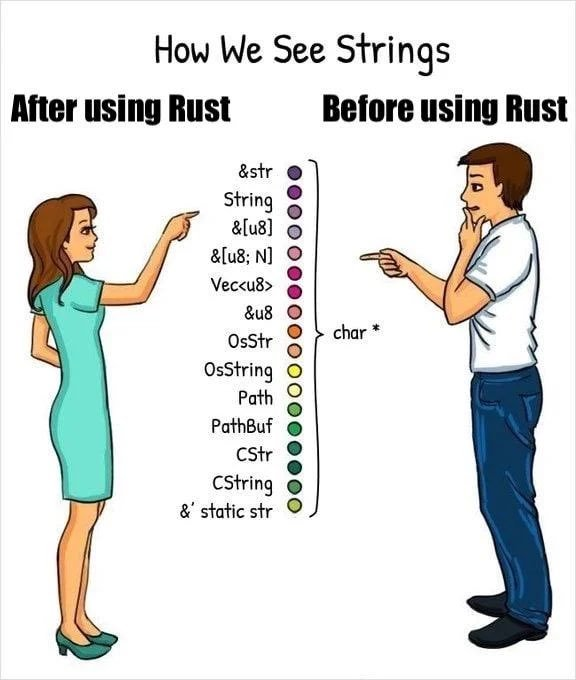
\includegraphics[height=5cm]{Img/typestr.jpg}
    \end{center}
  \end{columns}
\end{frame}

\begin{frame}[fragile]{Pattern matching}
  \begin{columns}[t]
    \column{0.6\textwidth}
    \begin{tcolorbox}[safebox, title={\faRust\ Enums avec données + Pattern Matching}]
      \begin{minted}[fontsize=\scriptsize]{rust}
enum Shape {
    Circle(f64),
    Rectangle(f64, f64),
}

let aire = match shape {
    Shape::Circle(r)   => /* aire cercle */,
    Shape::Rectangle(w,h) => /* aire rect */,
    // exhaustif : le compilo force tous les cas
}
      \end{minted}
    \end{tcolorbox}
    {\footnotesize En C~: enum = juste un entier.\\
    En Rust~: enum = \textbf{type algébrique} avec données.}
    \column{0.4\textwidth}
    \begin{center}
      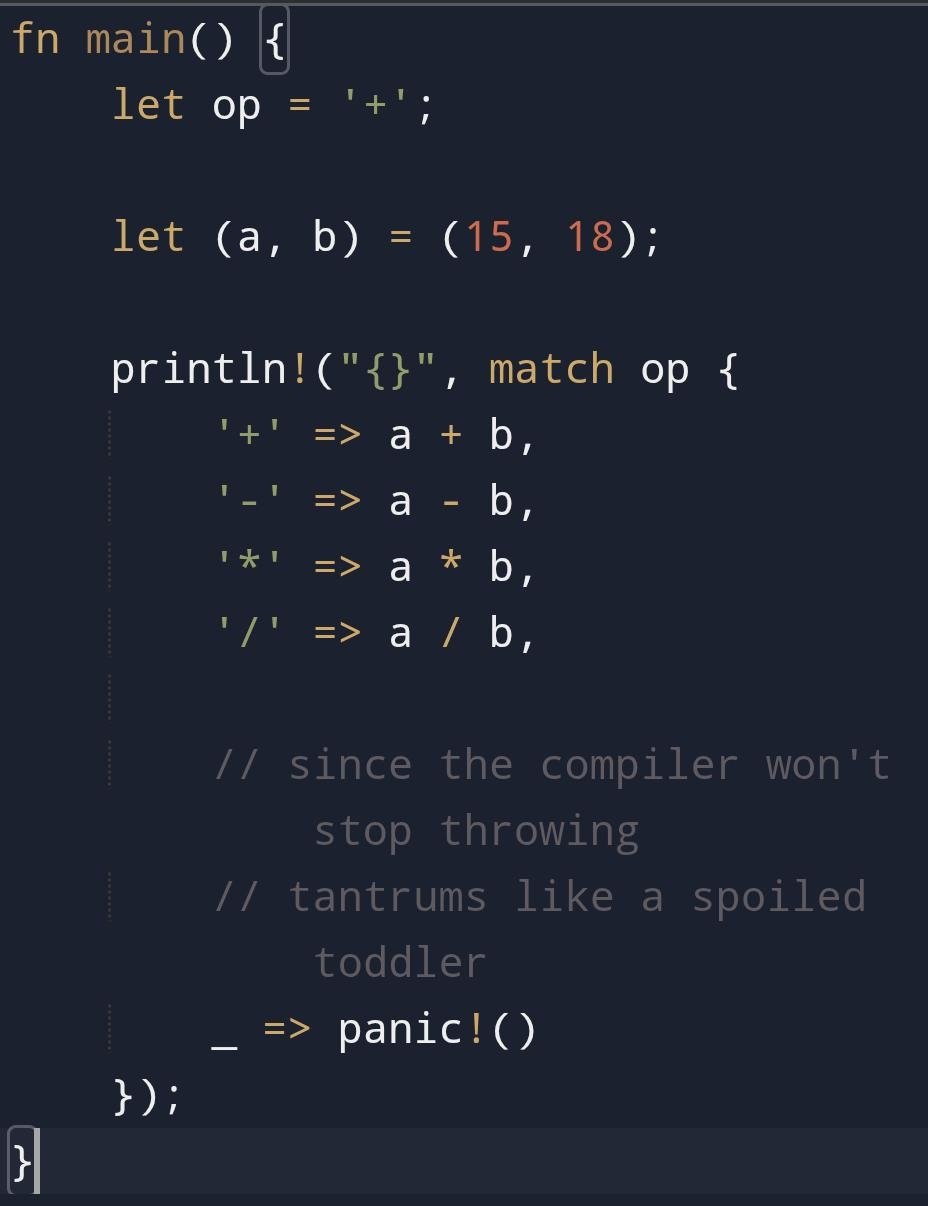
\includegraphics[height=5cm]{Img/patternmatching.jpeg}
    \end{center}
  \end{columns}
\end{frame}

\begin{frame}[fragile]{Variables immuables par défaut}
  \begin{columns}[t]
    \column{0.7\textwidth}
    \begin{block}{Immutable by default}
      \begin{minted}[fontsize=\scriptsize]{rust}
let x = 5;       // immutable par défaut
x = 6;           // ERREUR de compilation

let mut y = 5;   // mutable explicitement
y = 6;           // OK

struct Point {
    x: i32,
    y: i32,
}

let p = Point { x: 1, y: 2 }; // instance immutable par défaut
p.x = 10;                   // ERREUR de compilation

let mut p_mut = Point { x: 1, y: 2 }; // instance mutable
p_mut.x = 10;                         // OK
      \end{minted}
    \end{block}
    {\footnotesize En C~: tout est mutable sauf \ccode{const}.\\
    En Rust~: tout est immutable sauf \rust{mut}.
    $\to$ designs plus sûrs par défaut.}
  \end{columns}
\end{frame}

\begin{frame}[fragile]{\texttt{Option<T>}~--- Adieu le NULL}
  \begin{columns}[t]
    \column{0.48\textwidth}
    \begin{tcolorbox}[dangerbox, title={\faSkull\ NULL --- l'erreur à 1 milliard \$}]
      \small Tony Hoare (inventeur de \texttt{null})~:\\
      \textit{``I call it my billion-dollar mistake.''}\\[0.4em]
      Rust n'a \textbf{pas} de valeur \texttt{null}.\\
      À la place~: \rust{Option<T>}
    \end{tcolorbox}
    \vspace{0.3em}
    \begin{minted}[fontsize=\scriptsize]{rust}
enum Option<T> {
    Some(T), // il y a une valeur
    None,    // absence de valeur
}
    \end{minted}

    \column{0.48\textwidth}
    \begin{minted}[fontsize=\scriptsize]{rust}
fn find(v: &[i32], t: i32) -> Option<usize> {
    v.iter().position(|&x| x == t)
}

match find(&[1, 2, 3], 2) {
    Some(i) => println!("Index : {}", i),
    None    => println!("Pas trouvé"),
}
    \end{minted}
    \vspace{0.3em}
    \begin{tcolorbox}[notebox, title={\faLightbulb Attention}]
      \small Vous \textbf{ne pouvez pas} oublier de gérer le cas absent.\\
      Le compilateur vous y \textbf{force}.
    \end{tcolorbox}
  \end{columns}
\end{frame}

\begin{frame}[fragile]{\texttt{Result<T,E>}~--- Les erreurs sont des valeurs}
  \begin{columns}[t]
    \column{0.52\textwidth}
    \begin{minted}[fontsize=\scriptsize]{rust}
enum Result<T, E> {
    Ok(T),  // succès
    Err(E), // erreur avec détail
}

fn parse_int(s: &str) -> Result<i32, ParseIntError> {
    s.trim().parse()
}

match parse_int("42abc") {
    Ok(n)  => println!("Nombre : {}", n),
    Err(e) => println!("Erreur : {}", e),
}
    \end{minted}

    \column{0.44\textwidth}
    \begin{tcolorbox}[safebox, title={\faRust\ vs exceptions Java/Python}]
      \small
      \begin{itemize}
        \item Les erreurs sont dans la \textbf{signature}
        \item Impossible de les \textbf{ignorer} accidentellement
        \item L'opérateur \rust{?} propage élégamment
        \item Zéro overhead (pas de try/catch stack unwinding)
      \end{itemize}
    \end{tcolorbox}
    \vspace{0.3em}
    \begin{minted}[fontsize=\scriptsize]{rust}
// Propagation avec ?
fn process(s: &str) -> Result<i32, _> {
    let n = parse_int(s)?; // propage si Err
    Ok(n * 2)
}
    \end{minted}
  \end{columns}
\end{frame}

\begin{frame}[fragile]{Syntaxe de base}
  \begin{columns}[t]
    \column{0.8\textwidth}
    \begin{tcolorbox}[safebox]
      \begin{minted}[fontsize=\scriptsize]{rust}
fn main() {
    let mut vec = vec![1, 2, 3];            // Vector mutable
    vec.push(4);                            // ajouter un élément
    let x = 2;
    if x > 1 { println!("x > 1"); }          // if sans else
    match x {
        1 => println!("un"),
        2 => println!("deux"),
        _ => println!("autre"),
    }
    while let Some(v) = vec.pop() {         // while + pattern matching
        println!("pop: {}", v);
    }
    for i in 0..3 {                         // for sur plage
        println!("{}", i);
    }
    for v in [10, 20, 30].iter() {          // for sur slice
        println!("{}", v);
    }
}
      \end{minted}
    \end{tcolorbox}
  \end{columns}
\end{frame}

\begin{frame}[fragile]{impl\&Traits~--- De l'OOP dans rust ?}
  \begin{columns}[t]
    \column{0.52\textwidth}
    \begin{minted}[fontsize=\scriptsize]{rust}
trait Area {
    fn area(&self) -> f64;
}

struct Circle    { r: f64 }
struct Rectangle { w: f64, h: f64 }

impl Circle {
  pub fn new(r:f64) -> Self { Circle {r} }
}
impl Area for Circle {
    fn area(&self) -> f64 { PI * self.r * self.r }
}
impl Area for Rectangle {
    fn area(&self) -> f64 { self.w * self.h }
}

fn print_area<T: Area>(shape: &T) { // Generics+trait bound
    println!("{}", shape.area());
}
let circle = Circle::new(10.0);
print_area(circle);
    \end{minted}
    \column{0.44\textwidth}
    \begin{tcolorbox}[notebox, title={\faLightbulb\ Traits $\approx$ interfaces}]
      \small Comme les interfaces Java / Go\\
      Polymorphisme \textbf{sans héritage de classe} et monomorphization.
    \end{tcolorbox}
    \begin{center}
      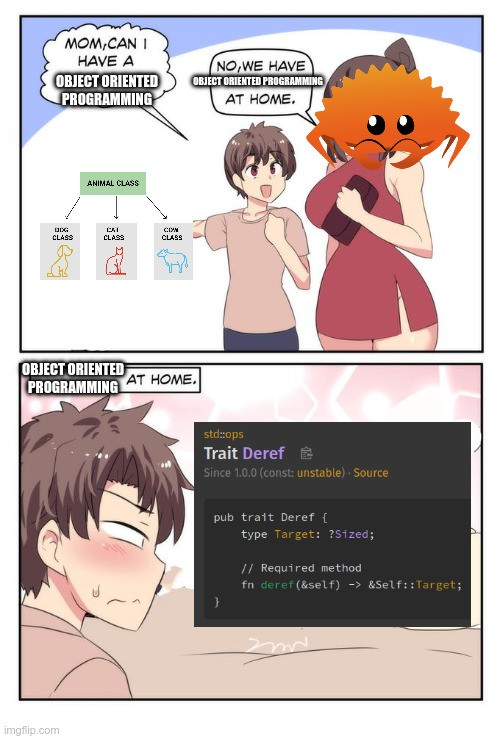
\includegraphics[height=4.73cm]{Img/oop.jpeg}
    \end{center}
  \end{columns}
\end{frame}

% ============================================================
\section{Écosystème}
% ============================================================

\begin{frame}[fragile]{Cargo~--- Le build system tout-en-un}
  \begin{columns}[t]
    \column{0.48\textwidth}
    \begin{tcolorbox}[dangerbox, title={En C~: l'enfer de configuration}]
      \small Make, CMake, Autotools, Conan, vcpkg\ldots\\
      Un projet, dix outils, zéro consensus.
    \end{tcolorbox}
    \vspace{0.3em}
    \begin{tcolorbox}[safebox, title={\faRust\ En Rust~: un seul outil}]
      \color{white}
      \begin{minted}[fontsize=\scriptsize]{bash}
cargo new mon_projet  # crée un projet
cargo build           # compile
cargo test            # lance les tests
cargo doc             # génère la doc
cargo add serde       # ajoute une dep
cargo clippy          # lint
cargo fmt             # formatte
      \end{minted}
    \end{tcolorbox}

    \column{0.47\textwidth}
    \begin{tcolorbox}[notebox, title={\faBoxOpen\ crates.io}]
      \small Registre de packages centralisé.\\
      \textbf{> 150~000 crates} disponibles.\\[0.3em]
      \mintinline{toml}{[dependencies]}\\
      \mintinline{toml}{regex = "1.0"}\\[0.3em]
      Résolution déterministe via \texttt{Cargo.toml} (analogue du \texttt{package.json} chez NodeJS)
    \end{tcolorbox}
    \vspace{0.3em}
    \begin{tcolorbox}[safebox, title={\faBook\ docs.rs}]
      \small Toute crate publiée~$\to$ documentation générée automatiquement.\\
      Les exemples dans la doc sont \textbf{testés} par \color{white} \bash{cargo test}
    \end{tcolorbox}
  \end{columns}
\end{frame}

\begin{frame}{rust-analyzer \& le compilateur qui vous aide}
  \begin{columns}[t]
    \column{0.6\textwidth}
    \begin{tcolorbox}[notebox, title={\faCode\ rust-analyzer}]
      \begin{itemize}\small
        \item Autocomplétion intelligente
        \item Navigation (go-to-def, find-refs)
        \item Refactoring assisté
        \item Documentation inline
        \item Erreurs en temps réel
      \end{itemize}
      \vspace{0.3em}
      VS Code, Neovim, IntelliJ\ldots
    \end{tcolorbox}
    \column{0.4\textwidth}
    \begin{center}
      
\includegraphics[height=5cm]{Img/rustanalyser.jpg}
    \end{center}
  \end{columns}
\end{frame}

\begin{frame}{rust-analyzer \& le compilateur qui vous aide}
  \begin{columns}[t]
    \column{0.5\textwidth}
    \begin{tcolorbox}[safebox, title={\faRust\ Un compilateur pédagogique}]
        \begin{itemize}\small
          \item Messages d'erreur \textbf{explicites} avec span précis
          \item Suggestions de correction concrètes
          \item \color{white}\bash{cargo clippy}\color{black}~: linter idiomatique
          \item \color{white}\bash{cargo fmt}\color{black}~: formatteur~-- pas de débats de style
          \item \color{white}\bash{cargo test}\color{black}~: tests unitaires intégrés
        \end{itemize}
    \end{tcolorbox}
    \column{0.5\textwidth}
    \begin{center}
      
\includegraphics[height=4cm]{Img/natives.jpg}
    \end{center}
  \end{columns}
  \begin{center}
    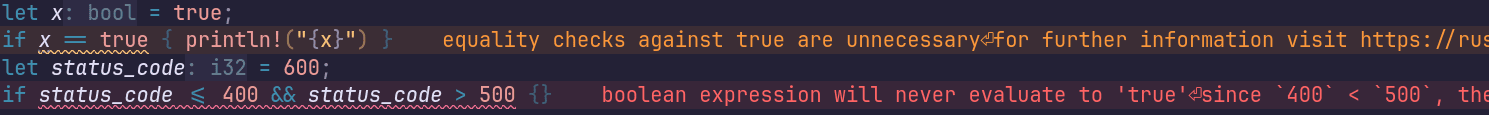
\includegraphics[width=18cm]{Img/clippy.png}
  \end{center}
\end{frame}

% ============================================================
\section{}
% ====================CONCLUSION====================

\begin{frame}{Ce qu'il faut retenir}
  \begin{columns}[t]
    \column{0.48\textwidth}
    \begin{tcolorbox}[rulebox, title={\faBrain\ Les 4 idées à retenir}]
      \begin{enumerate}\small
        \setlength\itemsep{0.5em}
        \item Rust n'est pas \textit{``du C avec plus de règles''}~---\\
              c'est un \textbf{modèle mémoire différent} encodé dans le système de types.
        \item Ownership + borrowing remplace le GC \textit{et} \ccode{free}
        \item Si ça compile~: toute une classe de bugs est \textbf{impossible}.
        \item L'écosystème (Cargo, rust-analyzer, clippy) et la stdlib sont d'une qualité rare pour un langage systèmes.
      \end{enumerate}
    \end{tcolorbox}

    \column{0.48\textwidth}
    \begin{tcolorbox}[dangerbox, title={\faExclamationCircle\ À mentionner}]
      \small \textbf{Unsafe Rust} existe~: blocs \rust{unsafe {}} pour les cas légitimes (FFI, optimisations hardcoded). C'est pour les fous.
    \end{tcolorbox}
    \begin{center}
      
\includegraphics[height=4.4cm]{Img/unsafe.jpg}
    \end{center}
  \end{columns}
\end{frame}

\begin{frame}[fragile]{Pour aller plus loin}
  \begin{columns}[t]
    \column{0.52\textwidth}
    \begin{block}{Ressources recommandées}
      \small
      \begin{tabular}{@{}ll@{}}
        \toprule
        \textbf{Ressource} & \textbf{Type} \\
        \midrule
        \href{https://doc.rust-lang.org/stable/book/}{The Rust Book} & Référence officielle \\
        \href{https://rust-book.cs.brown.edu}{Rust Book (Brown Univ.)} & Interactif + quizzes \\
        \href{https://github.com/rust-lang/rustlings}{Rustlings} & Exercices guidés \\
        \href{https://doc.rust-lang.org/rust-by-example/}{Rust by Example} & Snippets annotés \\
        \href{https://www.youtube.com/@jonhoo}{Jon Gjengset (YT)} & Vidéos avancées \\
        \href{https://www.youtube.com/@NoBoilerplate}{No Boilerplate (YT)} & Format court \\
        \bottomrule
      \end{tabular}
    \end{block}
    \begin{tcolorbox}[safebox]
      \small
      \textbf{Installer Rust~:}\\
      \texttt{curl --proto '=https' --tlsv1.2 -sSf https://sh.rustup.rs | sh}\\[0.4em]
      \textbf{Tester maintenant~:}\\
      \href{https://play.rust-lang.org}{play.rust-lang.org}\\
    \end{tcolorbox}
    \column{0.44\textwidth}
    \begin{center}
      
\includegraphics[height=6.5cm]{Img/learnrust.png}
    \end{center}
  \end{columns}
\end{frame}

% -------- QUESTIONS SLIDE -----------------------------------
{
\setbeamercolor{background canvas}{bg=RustDark}
\begin{frame}[plain]
  \begin{center}
    \vspace{2em}
    {\color{RustOrange}\fontsize{48}{56}\selectfont\faRust}\\[0.5em]
    {\color{white}\Huge\textbf{Questions~?}}\\[1em]
    {\color{RustLight}\large Slides + ressources disponibles sur mon github}\\[0.3em]
    {\color{RustOrange}\normalsize \faGithub\ \texttt{[github.com/Ilingu]}}
  \end{center}
\end{frame}
}

\end{document}
